\section{A noisy Markov chain is a tree}
\label{sec:tree}

\begin{figure}[t]
  \centering
  \begin{tikzpicture}[
    var/.style={circle,draw,thick,minimum size=8mm,inner sep=0pt},
    obs/.style={circle,draw,thick,fill=black!12,minimum size=8mm,inner sep=0pt},
    fac/.style={rectangle,fill=black,minimum size=2.4mm,inner sep=0pt},
    lab/.style={font=\small}]
  \foreach \i/\n in {0/1,1/2,2/3,3/L} {
    \node[var] (a\i) at (1.6*\i,0) {$a_{\n}$};
    \node[fac] (o\i) at (1.6*\i,-0.95) {};
    \node[obs] (x\i) at (1.6*\i,-1.9) {$x_{\n}$};
    \draw (a\i) -- (o\i) -- (x\i);
  }
  \foreach \i/\j in {0/1,1/2} {
    \node[fac] (k\i) at ($(a\i)!0.5!(a\j)$) {};
    \draw (a\i) -- (k\i) -- (a\j);
  }
  \draw (a2) -- ($(a2)!0.32!(a3)$);
  \node at ($(a2)!0.5!(a3)$) {$\cdots$};
  \draw ($(a2)!0.68!(a3)$) -- (a3);
  \node[lab,above=1.2mm of k1] {$K(a_3\,|\,a_2)$};
  \node[lab,right=1.2mm of o3] {$\ell_t(x_L\mid a_L)$};
  \draw[-{Stealth[length=2mm]},thick] ($(a0)+(-0.1,0.95)$) -- node[above,lab]{$\mu_{\to}$} ($(a1)+(0.3,0.95)$);
  \draw[-{Stealth[length=2mm]},thick] ($(a3)+(0.1,0.95)$) -- node[above,lab]{$\mu_{\leftarrow}$} ($(a2)+(-0.3,0.95)$);
\end{tikzpicture}

  \caption{\note{Factor graph of $p(a\mid x)$: kernel factors between neighbours, noise factors $\ell_t$ at each
  site; no loop, so BP is exact. Messages $\mu_\to$, $\mu_\leftarrow$. Slide 7.}}
  \label{fig:factor-graph}
\end{figure}

\note{J\'er\^ome (49:16): put the factor graph in, it shows at a glance that the model is a tree, which is not obvious
even to statistical physicists. BP at the level of his hierarchical-filtering paper \S2.4, ``maybe a bit more
detailed'' (48:37); BP on the grid is ``a bit detailed'' (50:20), so the grid recursions go to Appendix~A. Solve the
exactly known case here (12:01).}

\note{BP: forward and backward messages, marginal $\propto\mu_\to\mu_\leftarrow$, mean $\to$ score by
\cref{eq:tweedie}; any kernel, any $t$. On a grid: $N_g=401$ points, matrix--vector products, $O(LN_g^2)$.
Grid exactness: round-off on the Gaussian chain for $t\geq0.05$ (Appendix~A); about $10^{-5}$ on the Laplace chain.}

\begin{figure*}[t]
  \centering
  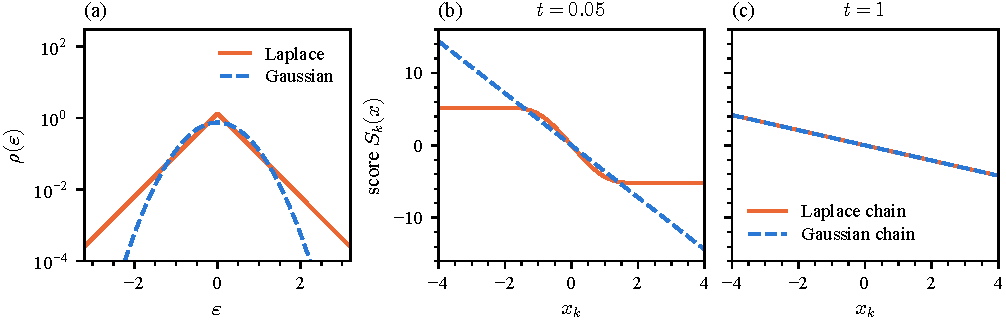
\includegraphics{fig_laplace}
  \caption{\note{(a) Laplace vs Gaussian innovation, same variance. (b, c) Score of the middle site against $x_k$ at
  $t=0.05$ and $t=1$: saturates at small noise, linear at large noise. Slide 6.}}
  \label{fig:laplace}
\end{figure*}

\begin{figure}[t]
  \centering
  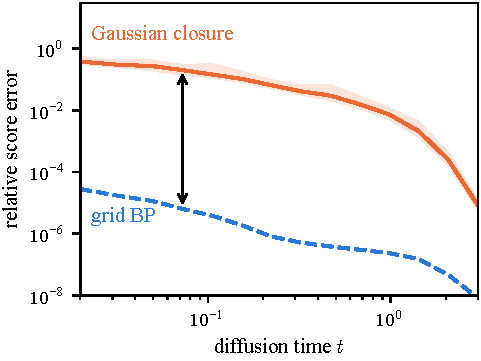
\includegraphics{fig_closure}
  \caption{\note{Laplace chain, true kernel: the best linear denoiser (Gaussian closure / Kalman) against grid BP's
  own error. Slide 8.}}
  \label{fig:closure}
\end{figure}

\note{Numbers: closure error median $0.27$ at $t=0.05$ ($0.38$ at $t=0.02$, $8\times10^{-6}$ at $t=3$) against grid
error $1.1\times10^{-5}$ --- thesis \texttt{tools/data/ch07\_metrics.csv}.}
